\section{Character of Energy and Electron Transfer Illustrated Using Pairs and Triples of Atoms}

\subsection{Distance Dependencies of ICD Decay Rates}



\subsection{Distance Dependencies of ETMD Decay Rates}
\textbf{Der Abstand zwischen den Atomen $A$ und $B$ $R_1$}:\\
$R_1$ erscheint nicht explizit in dem hergeleiteten asymtotischen Ausdruck für die Zerfallsbreiten, sondern implizit im Übergangsdipolmoment. Dieses nimmt exponentiell mit dem Abstand zwischen den Atomen ab.\\

\textbf{Der Abstand zwischen den Untereinheiten $AB$ und $C$ $R_2$}:\\
Wie zu erwarten war, hängt die Zerfallsbreite aufgrund der Energieübertragung durch eine Dipol-Dipol-Wechselwirkung mit $\frac{1}{R_2^6}$ vom Abstand der beiden Untereinheiten ab.\\


\subsection{Angle Dependencies of ETMD Decay Rates}
Consider the distances $R$ and $Q$ as definded in figure \ref{etmd_geom_pspic}
to be constant and the ratio between the transition dipole moments
in the $\tilde{z}$ and the $\tilde{x}$ direction
$q=\frac{|<\tilde{D}_x>|^2}{|<\tilde{D}_z>|^2}$ to be fixed to some number.
In this case the decay width for each $M_AB'$ has the angular dependence

\begin{align}
 \Gamma_i &\propto \left( 2q |<\tilde{D}_{z}>|^2 +
                  (4+2q)|<\tilde{D}_{z}>|^2 \cos^2\alpha +
                  (2+4q)|<\tilde{D}_{z}>|^2 \sin^2\alpha \right) \\
          &\propto 4q + 2 + 2 \cos^2\alpha + 2q \sin^2\alpha .
\end{align}

It is an oscillating function with the positions of maxima and minima
depending both on the ratio $q$ and the angle $\alpha$.

\begin{figure}[h]
 \centering
 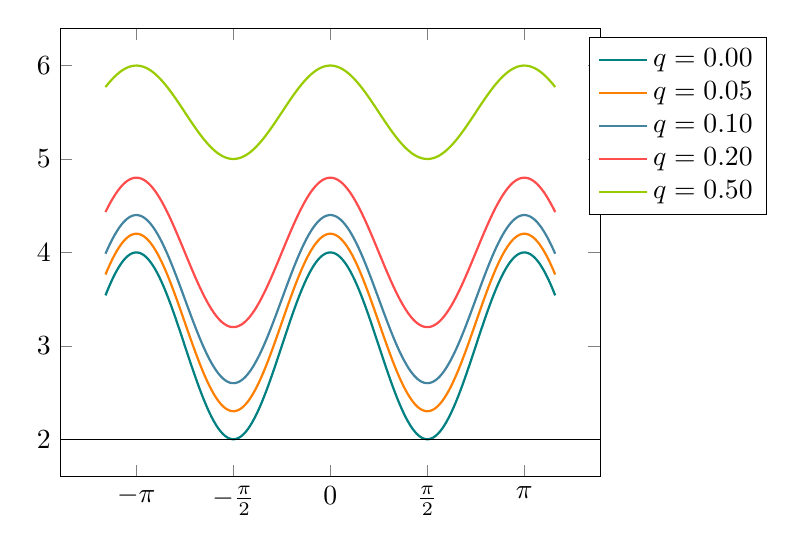
\begin{tikzpicture}
    \begin{axis}[%scale=0.8,
                 domain=-0.5-pi:0.5+pi,
                 samples = 200,
                 xtick={-3.14159,-1.57089,...,3.14159},
                 xticklabels={$-\pi$,$-\frac \pi 2$,0,$\frac \pi 2$,$\pi$},
                 cycle list name = exotic,
                 legend style={anchor= north west}
                 ]
    \foreach \q in {0.00,0.05,0.10,0.20,0.50}{
      \addplot+[mark = none,
               thick
               ]
               {4*\q + 2 + 2*cos(deg(x))^2 + 2*\q*sin(deg(x))^2}; 
      \addlegendentryexpanded{$q=\q$}
               }
      \draw[] (axis cs:\pgfkeysvalueof{/pgfplots/xmin},2) -- (axis cs:\pgfkeysvalueof{/pgfplots/xmax},2);
    \end{axis}
\end{tikzpicture}

 \caption{}
 \label{}
\end{figure}

In a real system, an energy transfer between
two dipoles is most efficient, if they are aligned in one direction.
Wihtin a dimer the most efficient electron transfer results in a
dipole aligned along the bonding axis and hence $q<1$. A typical
value of $q$ would be $\frac 1{10}$. In the 
case of $q$ approaching 0, the angular part of
the decay width
approaches a shifted $2\cos^2 \alpha$ with maxima at even multiples of $\frac \pi2$
and minima at uneven multiples of $\frac \pi2$ with values between
$4$ and $2$.
Therefore, for typical numbers of $q$ the energy transfer
to an atom on the same axis ($\alpha = 0,\pi$), corresponding
to a linear arrangement, is preferred.



\subsection{Influence of the Coordinate System Choice}
In section \ref{} a coordinate system was chosen to describe the
triatomic system. The distance $Q$ between the two atoms involved
in the energy transfer is reasonably defined. However, where the
center of the oscillating dipole moment of subsystem $S_1$ is, can
not unambigously be defined without further investigation. Most
probable it is somwhere between the atoms $A$ and $B$. Therefore
the center of mass was chosen to be the reference point for the
distance $R$ and associated with it the angle $\alpha$.
Another thinkable and for automatization of the calculation
convenient choice would be to anchorage $R$ and $\alpha$ at
atom $B$.
For the following discussion we will therefore refer to two sets
of coordinates of maximum deviation with origins residing in atoms
$A$ and $B$ with subscripts $A$ and $B$.

We assume that we have two constant distances $R_{A}$ and $R_B$
where either of these distances is larger than or equal to $Q$.
In this case the maximum and minimum of the ratio between the two
corresponding decay rates $\frac{\Gamma_{A}}{\Gamma_B}$ will occur
in the case of $\alpha = 0,\pi$ and $R_B = \frac 12 R_{A} = Q$
and $R_B = 2 R_{A} = 2Q$, respectively.

\begin{equation}
\text{minimum: } \frac{\Gamma_{A}}{\Gamma_B}= \frac{1}{64} \quad\quad
\text{maximum: } \frac{\Gamma_{A}}{\Gamma_B}= \frac{64}{1}
\end{equation}

From this we conclude, that the absolute numbers of calculated ETMD
decay widths are obviously error-prone. In the worst case the uncertainty
is given by factors $\frac{1}{64}$ or $\frac{64}{1}$.
In reality these worst cases will rarely be observed, since it on
the one hand is very unlikely to find two atoms at exactly the same place
and on the other hand ETMD preferably occurs at interfaces, which leads
to preferred angles higher than 0 and below $\pi$.
Additionally the larger the difference between $Q$ and $R$ become, the
smaller this effect is going to be.


\subsection{Relative Decay Rates Depending on the Symmetry of the Final States}
